\documentclass[t, aspectratio=169]{beamer}
\usepackage{scrextend}
\changefontsizes{16pt}
\usepackage[english]{babel}
\usepackage{textpos}

\usepackage{enumitem}
\setlist[description]{itemsep=0mm, topsep=0mm, itemindent=-4mm}

\title{Who's Julia?}
\author[simkn15, sonje15, asjen15]{simkn15, sonje15, asjen15}
\institute[Inst.]{\vspace*{-0.8cm}University of Southern Denmark}
\date{\vspace*{-0.8cm}\today}

\usetheme{Hannover}

\setbeamertemplate{frametitle}[default][left]

\begin{document}
\setbeamertemplate{footline}[text line]{
	\parbox{\linewidth}{\vspace*{-60pt}\hfill
\includegraphics[width=1.352cm,height=1.352cm]{img/sdu_segl.pdf}}}

	\begin{frame}
		\center
		
\includegraphics[height=2.704cm,width=4cm]{img/julia_small.png}
		\vspace*{-0.8cm}
		\maketitle
	\end{frame}
	
%Show our research
%
	
\setbeamertemplate{footline}[text line]{
	\parbox{\linewidth}{\vspace*{-60pt}
\includegraphics[height=1.352cm,width=2cm]{img/julia_200.png}\hfill\insertpagenumber\hfill
\includegraphics[width=1.352cm,height=1.352cm]{img/sdu_segl.pdf}}}
\setbeamertemplate{navigation symbols}{}
	\section{Julia}
	\begin{frame}
		\frametitle{Who's Julia}
		\begin{description}
			\item[$\cdot$] Under development since 2009
			\item[$\cdot$] Published 2012
			\item[$\cdot$] Newest stable version 0.4.5
			\item[$\cdot$] Open source
			\item[$\cdot$] Developers' goals
			\item[$\cdot$] Syntax
		\end{description}
	\end{frame}
	\section{Essential features}
	\begin{frame}
		\frametitle{Essential feature in Julia}
		\begin{description}
			\item[$\cdot$] Dynamic type system and package manager
			\item[$\cdot$] Calls to Python and C functions
			\item[$\cdot$] User-defined types
			\item[$\cdot$] Metaprogramming
			\item[$\cdot$] Garbage Collector
		\end{description}
	\end{frame}
	\section{Benchmarking}
	\begin{frame}
		\frametitle{Benchmarking}
		\begin{columns}[c] % the "c" option specifies center vertical alignment
		\column{.7\textwidth} % column designated by a command
		\begin{description}
			\item[$\cdot$] CPU time (user + system time)
			\item[$\cdot$] Profiling
		\end{description}
		\column{.3\textwidth}
			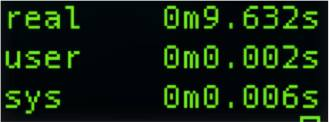
\includegraphics[height=1cm]{img/time.png}
		\end{columns}
	\end{frame}
	\section{Results}
	\begin{frame}
		\frametitle{Results}
	\end{frame}
	\section{Conclusion}
	\begin{frame}
		\frametitle{Conclusion}
	\end{frame}
\end{document}

